\documentclass[12pt]{article}
\usepackage{amsmath}
\usepackage{amsfonts}
\usepackage{amssymb}
\usepackage{physics}
\usepackage{graphicx}
\usepackage{hyperref}
\usepackage{subcaption}
\title{The Bethe-Salpeter Equation}
\author{Patryk Kozlowski}
\date{\today}
\begin{document}
\maketitle
\section{Mean field theory}
The central computational method in quantum chemistry is density functional theory (DFT). In their inaugural work, Hohenberg and Kohn proposed that the wave function for a system is uniquely determined by the electron density. Kohn and Sham then proposed a computational methodology that makes use of a self-consistent procedure, which is computationally cheap with a small scaling of $O(N^3)$, where $N$ is the number of electrons. It treats the quantum mechanical effects of the system by an exchange-correlation functional $V_{xc}$. This $V_{xc}$ is approximate and while you can get better ones by moving up Jacob's ladder, it is difficult to systematically improve due to what is known as the self-interaction error. Therefore, we turn to many-body perturbation theory (MBPT) which provides a framework to correct upon the properties predicted by DFT. In this work, we will consider the formalism of Green's functions within the framework of MBPT.
\section{Linear response theory}
When we interrogate the system with one beam as is done in linear spectroscopy, we are only interested in the response of properties, like the electron density, right after the perturbation of light. We can define a susceptibility $\chi$, which tells us how much the certain property will change in response to the perturbation. For example, we often think about how the polarization of the system will respond to a perturbation of light and we can write this polarization in terms of the susceptibility
\begin{equation}
P(\omega) = \chi(\omega)E(\omega),
\end{equation}
where $P$ is the polarization, $E$ is the electric field of the light, and $\omega$ is the frequency of the light. However, when wcne have only considered a linear susceptibility $\chi^{(1)}$ and in order to predict what will happen to the system with more interactions by light, as is done in nonlinear experiments, we want to compute the higher-order susceptibilities. This can be done with MBPT.

\section{Green's functions}
One can define the single-particle interacting Green's function $G$ as
\begin{equation}
G\left(\mathbf{r}_1, t_1 ; \mathbf{r}_2, t_2\right)=-i\left\langle\Psi_0\left|T\left[\psi\left(\mathbf{r}_1, t_1\right) \psi^{\dagger}\left(\mathbf{r}_2, t_2\right)\right]\right| \Psi_0\right\rangle,
\end{equation}
where $\psi$ is the field operator for creating or destroying a particle at spacetime coordinates $\mathbf{r}$ and $t$, $T$ is the time-ordering operator that ensures that the $\psi$ at the earlier time is acting on the ket before the $\psi$ at the later time, and $\Psi_0$ is the ground state wave function. The Green's function can be interpreted as measuring the probability that a particle created at $\mathbf{r}_2$ and $t_2$ will be destroyed at $\mathbf{r}_1$ and $t_1$. In the same vein, one can define the single-particle noninteracting Green's function $G_0$ as
\begin{equation}
G_0\left(\mathbf{r}_1, t_1 ; \mathbf{r}_2, t_2\right)=-i\left\langle\Phi_0\left|T\left[\psi\left(\mathbf{r}_1, t_1\right) \psi^{\dagger}\left(\mathbf{r}_2, t_2\right)\right]\right| \Phi_0\right\rangle,
\end{equation}
The only difference is that here we are dealing with the field operators and ground state wave function $\Phi_0$ of the noninteracting system. An explanation of why we use the distinction between noninteracting and interacting Green's functions is in short order, but in the meantime, this can be understood as the difference between a mean field theory, like DFT, and the MBPT, that has been used to correct it. We can write down a Dyson equation, which relates the noninteracting Green's to the interacting one
\begin{equation}
G=G_0+G_0\Sigma G,
\label{eq:dyson}
\end{equation}
where we have introduced $\Sigma$, which is the self-energy operator. As one can see, the self-energy effectively provides the difference between the noninteracting system and the fully interacting one. The self-energy admits an intuitive physical picture. Consider the example of an electron shot into a gas of electrons, as shown in Figure \ref{fig:shot}.
\begin{figure}
\begin{subfigure}{.5\textwidth}
  \centering
  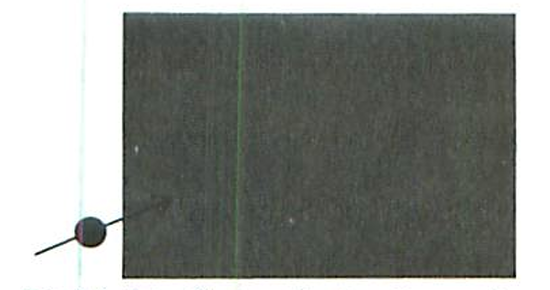
\includegraphics[width=.8\linewidth]{shot.png}
  \caption{The electron is shot into the gas}
  \label{fig:shot}
\end{subfigure}
\begin{subfigure}{.5\textwidth}
  \centering
  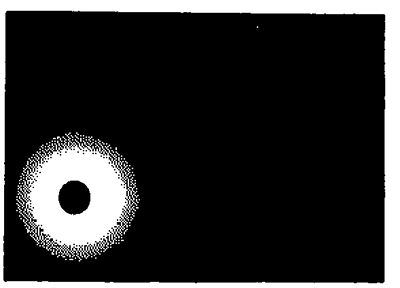
\includegraphics[width=.8\linewidth]{clothing.png}
  \caption{The electron creates holes as it moves along}
  \label{fig:clothing}
\end{subfigure}
\caption{Electron gas propagation taken from}
\label{fig:propagates}
\end{figure}
As it propagates through this medium, it will have an electrostatic repulsion with the electrons in the gas, so it will create holes (depicted in white) as it moves along (pictured in Figure \ref{fig:clothing}). Therefore, it no longer makes sense to think of the bare electron, but rather the quasi-electron along with its "clothing" of holes. To make this more rigorous, we have the equation
\begin{equation}
    \epsilon_{\text{quasi}} - \epsilon_{\text{bare}} = \epsilon_{\text{self}},
\end{equation}
which is saying that the difference between the quasi-electron energy and the bare electron energy can be thought of as the electron's self-energy, or just the energy of its "clothing". So we can think of $\epsilon_{\text{bare}}$ and $\epsilon_{\text{quasi}}$ as originating from the noninteracting and interacting Green's functions $G_0$ and $G$, respectively. The self-energy $\Sigma$ then captures the difference between these two quantities. Typically, $\Sigma$ is designed to capture all of the quantum mechanical effects of the many-body system, including the exchange and correlation effects, so it is often denoted as $\Sigma_{xc}$. One might argue that DFT also contains a $V_{xc}$, but this is often an approximation that doesn't work universally for systems, whereas the $\Sigma_{xc}$ can be systematically improved by considering increasing orders of perturbation theory.
\section{The $GW$ approximation}
In order to solve the Dyson equation in \ref{eq:dyson}, we need to make approximations of the self-energy $\Sigma$. By introducing the screened Coulomb potential $W$, which represents the effective electrostatic interaction between electrons (as described above through the concept of the quasi-electron), the polarization function $P$, which describes the response of the system to the introduction of an electron, and the vertex function $\Gamma$, which describes the interaction between the electrons and holes, we can write down the five Hedin's equations
\begin{equation}
\begin{aligned}
& G(1,2)=G_0(1,2)+\int d(3,4) G_0(1,3) \Sigma(3,4) G(4,2) \\
& P(1,2)=\int d(3,4) G(1,3) G(4,2) \Gamma(3,4 ; 2) \\
& W(1,2)=V(1,2)+\int d(3,4) V(1,3) P(3,4) W(4,2) \\
& \Sigma(1,2)=\int d(3,4) G(1,3) \Gamma(3,2 ; 4) W(4,1) \\
& \Gamma(1,2 ; 3)=\delta(1,2) \delta(1,3)+\int d(4,5,6,7) \frac{\delta \Sigma(1,2)}{\delta G(4,5)} G(4,6) G(7,5) \Gamma(6,7 ; 3)
\end{aligned}
\end{equation}
where we have made use of the shorthand notation $1=(\mathbf{r}_1, t_1)$ and $V$ is the bare Coulomb potential. The $GW$ approximation is a simplification of these equations, where we neglect the vertex function $\Gamma$ by setting $\Gamma (1,2,3)= \delta (1,2) \delta (1,3)$. This simplifies the equations for the self-energy and polarization function to
\begin{equation}
\begin{aligned}
& \Sigma(1,2)=\int d(1,2) G(1,2) W(1,2) \\
& P(1,2)=\int d(1,2) G(1,2) G(2,1). \\
\end{aligned}
\end{equation}
\begin{figure}
    \centering
    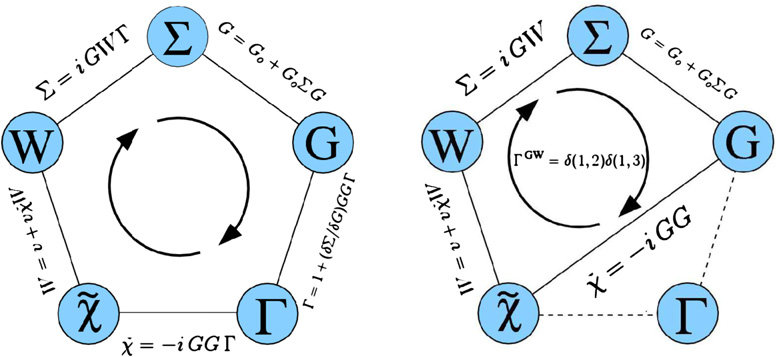
\includegraphics[width=\textwidth]{Left-panel-Graphical-representation-of-Hedins-equations-Right-panel-The-four-coupled.jpg}
    \caption{Graphical representation of Hedin's equations. The left panel shows the full set of equations, whereas the right panel shows the $GW$ approximation.}
    \label{fig:hedin}
\end{figure}
The figure \ref{fig:hedin} shows the self-consistency between these equations, with the polarization $P$ represented by $\tilde{\chi}$. Full self-consistency, including the vertex function $\Gamma$, is shown in the left panel, whereas the $GW$ approximation, which neglects the vertex function, is shown in the right panel.
\section{The Bethe-Salpeter equation}
Now comes the Bethe-Salpeter equation, which includes the vertex function $\Gamma$ within this self-consistent cycle.
\end{document}